%Write about analysis and preprocessing here
\section{Data analysis}
The data we use is a subset of Netflix Prize data. The data consists
of ratings for 17770 movies. There are ratings from 3255352 users in
the training set and 100478 users in the tests set (data computed from
the line count of TrainingRatings.txt, TestingRatings.txt and
movie\_titles.txt). The size of the problem indicates that cloud
computing is necessary.

For a better algorithm design, we first performed analysis to the
dataset with Spark. A random subset of the data is drawn for the
analysis, see Table~\ref{tab:subsample} for the size of sampled
data. The analysis gives us the answer of the following problems:

\begin{table}
  \centering
  \begin{tabular}{| p{5cm} | p{3cm} | p{3cm} |}
      \hline
       & Movie & User \\
      \hline
      Training set & 1821 & 28978\\
      \hline
      Testing set & 1701 & 27555\\
      \hline
  \end{tabular}
  \caption{The size of sampled data for analysis}
  \label{tab:subsample}
\end{table}

\subsection*{Similarity measurement}
The first key design choice is which similarity measurement to use for
the $kth$ nearest neighbor search. To this end, we compute the
histogram of average user ratings of the training set, see
Figure~\ref{fig:hist}.
\begin{figure}[!ht]
  \centering
  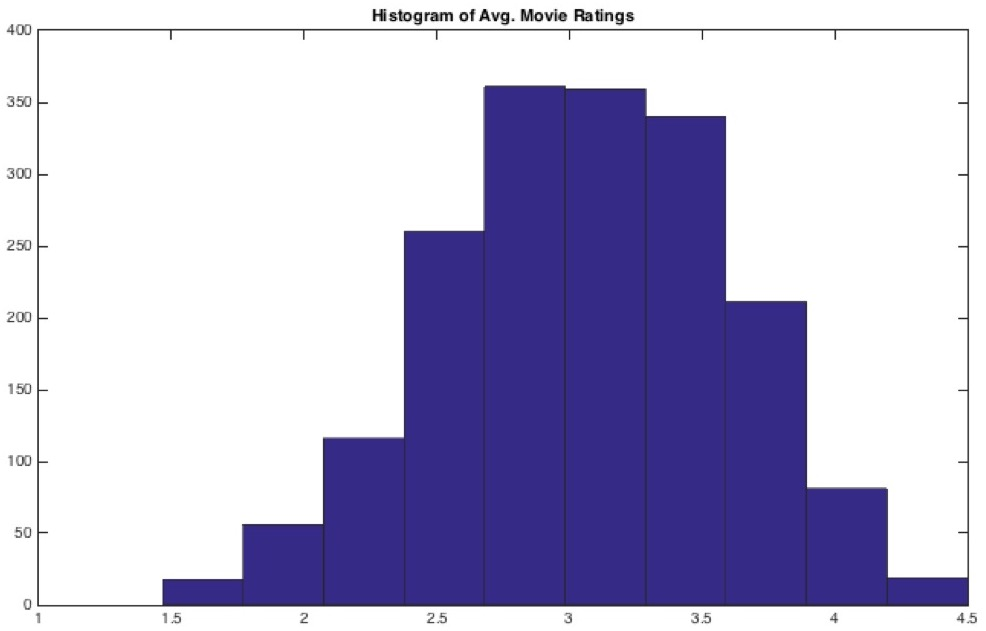
\includegraphics[width=0.8\textwidth]{images/hist}
  \caption{Histogram of average user ratings in the training set}
  \label{fig:hist}
\end{figure}

The result suggests that most users rate normally. Therefore, we
choose to use cosine similarity rather than Pearson similarity for
efficiency.

\subsection*{User-user similiary vs. movie-movie similarity}
To fill the missing entry, we can either use user as the key and fill with
ratings of other similar users, or we can use movie as the key and
fill with ratings of other similar movies. The choice depends of the
expected overlay of users in test and train and items in test and
train. See Table~\ref{tab:overlay}.

\begin{table}[!ht]
  \centering
  \begin{tabular}{|p{5cm}|p{5cm}|}
    \hline
    user-user & movie-movie\\
    \hline
    0.125467 & 0.439962\\
    \hline
  \end{tabular}
  \caption{Expected overly of two different keys}
  \label{tab:overlay}
\end{table}

The result suggests that use movie-movie similarity is more
appropriate.

\subsection*{Memory consumption}
The algorithm will use two MapReduce jobs: the first job computes
the list of users that rate each movie, and the second job computes
the similarity of each pair of movies. The memory bottleneck happens
at the reducer of each job. For first job, the expected memory usage
is 111.5589MB and for the second job, the expected memory usage is 4.4MB.

To summarize, we decided to implement an algorithm that first compute
movies that have similar user ratings with the query entry, then
predict the rating of the entry with known ratings from the similar
movie. The similarity is measured by Cosine similarity.
